\documentclass[a4paper, 12pt]{article}
\usepackage{pgfplots, mathtools}

%% Listings With Code-Styling and Grey Background
\usepackage{float, listings} 
\lstset{						% Global Listing settings
	language=Verilog,
	numbers=left,
	numberstyle=\tiny\color{gray},
%	firstnumber=1,
	numberfirstline=true,
	stepnumber=1,
	tabsize=2,
	breaklines=true,
}
\usepackage{xcolor, mdframed, graphicx}
\definecolor{code-gray}{gray}{0.93}

%% Make specific pages landscale for larger figures
\usepackage{pdflscape}

%% Custom FSM's
\usepackage{tikz}
\usetikzlibrary{automata, positioning, arrows, positioning}
\tikzset{very thick, ->, >=stealth', node distance=6cm, every state/.style={thick, fill=gray!10}, initial text=$ $}

%% Automatic Word Formatting
\usepackage{xspace}
\newcommand*{\Vivado}{\textit{Vivado}\xspace} % Italicize Vivado
\newcommand*{\SV}{\textbf{SystemVerilog}\xspace} % Bold SystemVerilog

%% Clickable links in the output PDF
\usepackage{hyperref}
\hypersetup{colorlinks=true, linktoc=all, linkcolor=black}

%% Figure Numbering Within Sections
\let\counterwithout\relax
\let\counterwithin\relax
\usepackage{chngcntr}
\counterwithin{figure}{section}

%% Macros for logic timing diagrams
\newcounter{wavenum}
\setlength{\unitlength}{1cm}
% advance clock one cycle, not to be called directly
\newcommand*{\clki}{
  \draw (t_cur) -- ++(0,.3) -- ++(.5,0) -- ++(0,-.6) -- ++(.5,0) -- ++(0,.3)
    node[time] (t_cur) {};
}
\newcommand*{\bitvector}[3]{
  \draw[fill=#3] (t_cur) -- ++( .1, .3) -- ++(#2-.2,0) -- ++(.1, -.3)
                         -- ++(-.1,-.3) -- ++(.2-#2,0) -- cycle;
  \path (t_cur) -- node[anchor=mid] {#1} ++(#2,0) node[time] (t_cur) {};
}
% \known{val}{length}
\newcommand*{\known}[2]{
    \bitvector{#1}{#2}{white}
}
% \unknown{length}
\newcommand*{\unknown}[2][XXX]{
    \bitvector{#1}{#2}{black!20}
}
% \bit{1 or 0}{length}
\newcommand*{\bit}[2]{
  \draw (t_cur) -- ++(0,.6*#1-.3) -- ++(#2,0) -- ++(0,.3-.6*#1)
    node[time] (t_cur) {};
}
% \unknownbit{length}
\newcommand*{\unknownbit}[1]{
  \draw[ultra thick,black!50] (t_cur) -- ++(#1,0) node[time] (t_cur) {};
}
% \nextwave{name}
\newcommand{\nextwave}[1]{
  \path (0,\value{wavenum}) node[left] {#1} node[time] (t_cur) {};
  \addtocounter{wavenum}{-1}
}
% \clk{name}{period}
\newcommand{\clk}[2]{
    \nextwave{#1}
    \FPeval{\res}{(\wavewidth+1)/#2}
    \FPeval{\reshalf}{#2/2}
    \foreach \t in {1,2,...,\res}{
        \bit{\reshalf}{1}
        \bit{\reshalf}{0}
    }
}

% \begin{wave}[clkname]{num_waves}{clock_cycles}
\newenvironment{wave}[3][clk]{
  \begin{tikzpicture}[draw=black, yscale=.7,xscale=1]
    \tikzstyle{time}=[coordinate]
    \setlength{\unitlength}{1cm}
    \def\wavewidth{#3}
    \setcounter{wavenum}{0}
    \nextwave{#1}
    \foreach \t in {0,1,...,\wavewidth}{
      \draw[dotted] (t_cur) +(0,.5) node[above] {t=\t} -- ++(0,.4-#2);
      \clki
    }
}{\end{tikzpicture}}

%$ Specific Line Breaks
% See https://tex.stackexchange.com/questions/26174/ for details
\usepackage[british]{babel} 

%% Page Margins
\usepackage[margin=1.00in]{geometry}

%% Beginning of Document
\begin{document}
\counterwithin{lstlisting}{section} % Listings are numbered within sections
% Title
\title{ECE 440 - Project \#3}
\author{Collin Heist}
\date{\today}
\maketitle

% Table of Content and Listings
\pagenumbering{roman}
\tableofcontents
\renewcommand{\listfigurename}{Figures}
\listoffigures
\lstlistoflistings
\newpage
\pagenumbering{arabic}

% Beginning of Report
\section{Design}
\subsection{Wrapper Block Diagram}
As part of \textbf{Homework \#4}, and for the purpose of clearly outlining the necessary components for my wrapper, I designed the following block diagram for the overall wrapper module.

\begin{figure}[h]
\hspace*{-0.75cm}
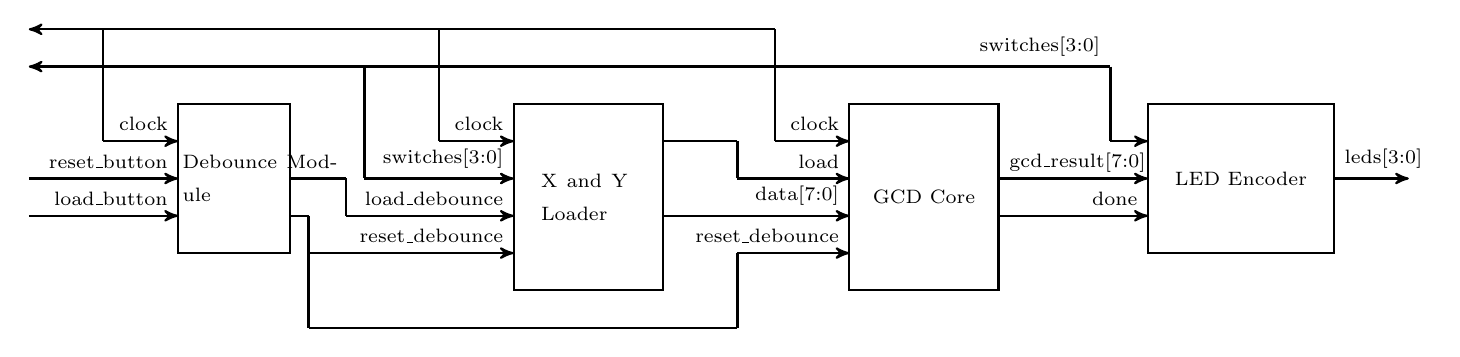
\begin{tikzpicture}[thick, node distance=0.5cm]
\def \scale {18/38}

\draw[<-] (0, -0) -- (20*\scale, -0);
\draw[<-] (0, -1*\scale) -- (29*\scale, -1*\scale) node[above left]{\scriptsize{switches[3:0]}};
\draw[-] (2*\scale, -0) -- (2*\scale, -3*\scale);
\draw[->] (2*\scale, -3*\scale) -- (4*\scale, -3*\scale) node[above left]{\scriptsize{clock}};
\draw[->] (0, -4*\scale) -- (4*\scale, -4*\scale) node[above left]{\scriptsize{reset\_button}};
\draw[->] (0, -5*\scale) -- (4*\scale, -5*\scale) node[above left]{\scriptsize{load\_button}};
\draw (4*\scale, -2*\scale) rectangle (7*\scale, -6*\scale) node[midway, text width=2cm, xshift=0.35cm]{\scriptsize{Debounce Module}};
\draw[-] (11*\scale, 0*\scale) -- (11*\scale, -3*\scale);
\draw[->] (11*\scale, -3*\scale) -- (13*\scale, -3*\scale) node[above left]{\scriptsize{clock}};
\draw[-] (9*\scale, -1*\scale) -- (9*\scale, -4*\scale);
\draw[->] (9*\scale, -4*\scale) -- (13*\scale, -4*\scale) node[above left]{\scriptsize{switches[3:0]}};
\draw[-] (7*\scale, -4*\scale) -- (8.5*\scale, -4*\scale);
\draw[-] (8.5*\scale, -4*\scale) -- (8.5*\scale, -5*\scale);
\draw[->] (8.5*\scale, -5*\scale) -- (13*\scale, -5*\scale) node[above left]{\scriptsize{load\_debounce}};
\draw[-] (7*\scale, -5*\scale) -- (7.5*\scale, -5*\scale);
\draw[-] (7.5*\scale, -5*\scale) -- (7.5*\scale, -8*\scale);
\draw[-] (7.5*\scale, -8*\scale) -- (19*\scale, -8*\scale);
\draw[->] (7.5*\scale, -6*\scale) -- (13*\scale, -6*\scale) node[above left]{\scriptsize{reset\_debounce}};
\draw (13*\scale, -2*\scale) rectangle (17*\scale, -7*\scale) node[midway, text width=2cm, xshift=0.4cm]{\scriptsize{X and Y Loader}};
\draw[-] (20*\scale, 0) -- (20*\scale, -3*\scale);
\draw[->] (20*\scale, -3*\scale) -- (22*\scale, -3*\scale) node[above left]{\scriptsize{clock}};
\draw[-] (17*\scale, -3*\scale) -- (19*\scale, -3*\scale);
\draw[-] (19*\scale, -3*\scale) -- (19*\scale, -4*\scale);
\draw[->] (19*\scale, -4*\scale) -- (22*\scale, -4*\scale) node[above left]{\scriptsize{load}};
\draw[->] (17*\scale, -5*\scale) -- (22*\scale, -5*\scale) node[above left]{\scriptsize{data[7:0]}};
\draw[-] (19*\scale, -8*\scale) -- (19*\scale, -6*\scale);
\draw[->] (19*\scale, -6*\scale) -- (22*\scale, -6*\scale) node[above left]{\scriptsize{reset\_debounce}};
\draw (22*\scale, -2*\scale) rectangle (26*\scale, -7*\scale) node[midway]{\scriptsize{GCD Core}};
\draw[-] (29*\scale, -1*\scale) -- (29*\scale, -3*\scale);
\draw[->] (29*\scale, -3*\scale) -- (30*\scale, -3*\scale);
\draw[->] (26*\scale, -4*\scale) -- (30*\scale, -4*\scale) node[above left, xshift=3, yshift=-1.5]{\scriptsize{gcd\_result[7:0]}};
\draw[->] (26*\scale, -5*\scale) -- (30*\scale, -5*\scale) node[above left]{\scriptsize{done}};
\draw (30*\scale, -2*\scale) rectangle (35*\scale, -6*\scale) node[midway]{\scriptsize{LED Encoder}};
\draw[->] (35*\scale, -4*\scale) node[above right]{\scriptsize{leds[3:0]}} -- (37*\scale, -4*\scale) ;
\end{tikzpicture}
\label{fig:block-diagram}
\end{figure}

The debounce module was provided for us, and the logic for the \textbf{X and Y Loader} is outlined in \textbf{Section~\ref{subsec:wrapper-fsm}}. The GCD core is the unchanged code from \textbf{Project \#2}, and the LED encoder is purely combinational and is described in \textbf{Section~\ref{subsec:led-encoder}}.

\subsection{Wrapper Input Selection Finite State Machine}
\label{subsec:wrapper-fsm}
I decided to implement the input logic using a very basic finite state machine. Sequentially selecting \textbf{X} and \textbf{Y} could not be done without sequential logic because the previous presses of \textbf{BTN1} must be remembered. 

The FSM I implemented in \textbf{Listing~\ref{lst:wrapper}} is shown below:

\begin{figure}[H]
\centering
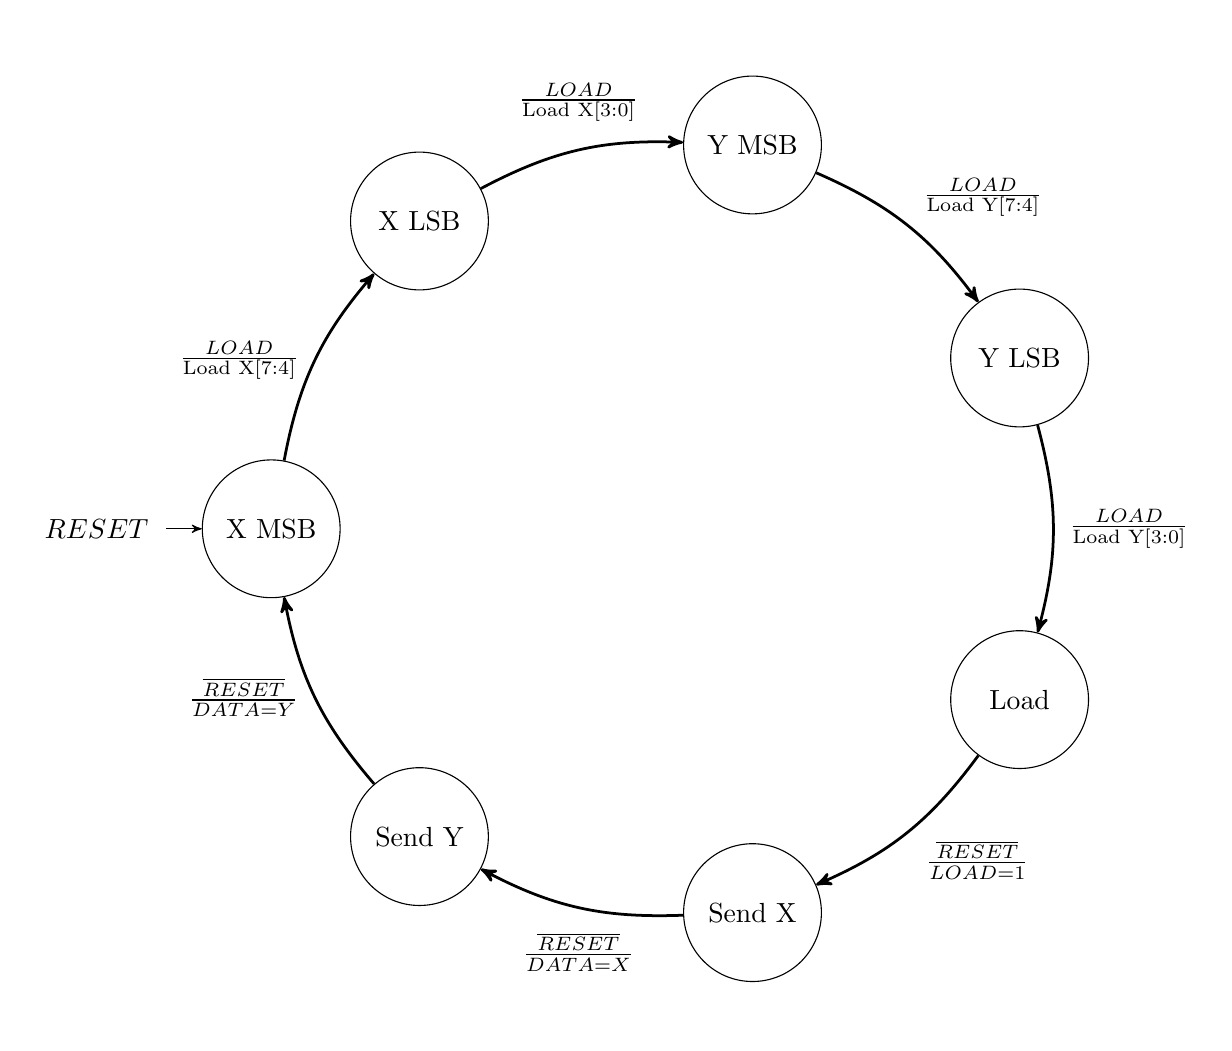
\begin{tikzpicture}[initial text=$RESET$, every node/.style={circle, minimum size=1.75cm}]
	\def \curv {15} %15 seems good
	\node[initial, draw] at ({360/7*(1-1)}:-5cm) (X MSB) {X MSB};
	\node[draw] at ({360/7*(1-2)}:-5cm) (X LSB) {X LSB};
	\node[draw] at ({360/7*(1-3)}:-5cm) (Y MSB) {Y MSB};
	\node[draw] at ({360/7*(1-4)}:-5cm) (Y LSB) {Y LSB};
	\node[draw] at ({360/7*(1-5)}:-5cm) (Load) {Load};
	\node[draw] at ({360/7*(1-6)}:-5cm) (Send X) {Send X};
	\node[draw] at ({360/7*(1-7)}:-5cm) (Send Y) {Send Y};
	\draw[->, line width=0.35mm]
		(X MSB) edge[bend left=\curv, left] node{$\frac{LOAD}{\text{Load X[7:4]}}$} (X LSB)
		(X LSB) edge[bend left=\curv, above] node[yshift=-10]{$\frac{LOAD}{\text{Load X[3:0]}}$} (Y MSB)
		(Y MSB) edge[bend left=\curv, right] node[yshift=10]{$\frac{LOAD}{\text{Load Y[7:4]}}$} (Y LSB)
		(Y LSB) edge[bend left=\curv, right] node{$\frac{LOAD}{\text{Load Y[3:0]}}$} (Load)
		(Load) edge[bend left=\curv, right] node[yshift=-10]{$\frac{\overline{RESET}}{LOAD=1}$} (Send X)
		(Send X) edge[bend left=\curv, below] node[yshift=10]{$\frac{\overline{RESET}}{DATA=X}$} (Send Y)
		(Send Y) edge[bend left=\curv, left] node{$\frac{\overline{RESET}}{DATA=Y}$} (X MSB);
\end{tikzpicture}
\caption{Input Finite State Machine}
\label{fig:fsm}
\end{figure}

This FSM was implemented inside a sequential block, with the \textbf{LOAD} signal being used to begin many of the state transitions referencing the output of the button debouncer. This was necessary in order to avoid loading the registers with all of the same value (triggered by many debounces).

This state mechanism interacts with the \textbf{gcd\_core} module, and the final three states are input-independent (excluding reset, obviously) that only exist to send the \textbf{Load}, \textbf{X}, and \textbf{Y} signals synchronized with the clock. Because of this, there is no need to send the debounced load signal directly into the GCD core module, as four load-button presses will automatically trigger the only required load into the module.

\subsection{LED Encoder}
\label{subsec:led-encoder}
As shown in \textbf{Figure~\ref{fig:block-diagram}}, the output logic is purely combinational, and is dependent upon the status of the switches and the constantly-asserted \textbf{Done} signal from the GCD Core. Because of this, the implementation for this section was very simple, and shown at the end of \textbf{Listing~\ref{lst:wrapper}}, specifically lines 84-95.

\section{Tribulations}
\label{sec:tribulations}
My first implementation of the FSM in \textbf{Figure~\ref{fig:fsm}} had the debounced load being required for all state transitions, not just the first four \textit{loading} states. This seemed necessary to me at first, as button presses were necessary for advancing the FSM at first, but upon simulating this with my testbench (see \textbf{Listing~\ref{lst:testbench}}), I noticed that the FSM never went past the \textbf{Send X} state. This of course makes sense, because the user is not required to press any more buttons after both X and Y are loaded, and so the transitions to send X and Y over the \textbf{Data} line never occurred. This was fixed by changing my FSM code to include a second if statement checking only if reset was not asserted, and if the state was already on the \textbf{Send Load} state, then transitions occurred on all clock edges.

The next problem I encountered occurred while I was testing my code on the hardware. I was not able to \textit{randomly} generate suitable numbers that had a high-enough GCD to verify that toggling between seeing the MSB or LSB of the result was working. For my simulations I only tested (at that point) relatively small numbers with GCD's less than $2^4$. To rectify this I wrote a small Python script to test all possible number combinations between 1 and $2^8$ and output the ones with the highest GCD. This gave me the inputs of $x=236$, and $y=156$ with a GCD of 78 ($|0100|1110|$ in binary) - achievable in a relatively small amount of operations on the datapath. This allowed me to verify that my MSB and LSB toggle was working properly.

\begin{landscape}
\section{Simulations}
\subsection{Behavioral Simulation}
After addressing those issues detailed in \textbf{Section~\ref{sec:tribulations}}, my behavioral simulation went exactly as expected, and is shown in \textbf{Figure~\ref{fig:behav-sim}}.

\begin{figure}[H]
\centering
\includegraphics[width=0.65\paperheight, keepaspectratio=true]{Sources/Behav-Sim.PNG}
\caption{Behavioral Simulation.}
\label{fig:behav-sim}
\end{figure}

\subsection{Post-Synthesis Timing Simulation}
With a lot of the information obfuscated, the post-synthesis simulation is a lot smaller, but shows the same results as the behavioral. 

\begin{figure}[H]
\centering
\includegraphics[width=0.80\paperheight, keepaspectratio=true]{Sources/Post-Synth-Timing-sim.PNG}
\caption{Post-Synthesis Timing Simulation.}
\label{fig:post-synth-sim}
\end{figure}

This is as-expected, with the exception of the small \textit{blip} on \textbf{leds[0]} for approximately 75 picoseconds. After verifying the logic was sound, and ensuring this behavior was not present when implemented on the board, I determined this was due to some combinational logic delays, and was small-enough to be ignored.
\end{landscape}

\section{Source Code}
\begin{mdframed}[backgroundcolor=code-gray, roundcorner=10pt, innerleftmargin=25, innertopmargin=5, innerbottommargin=5]	
\lstinputlisting[caption=Wrapper Module, label={lst:wrapper}]{Sources/wrapper.sv}
\end{mdframed}

\begin{mdframed}[backgroundcolor=code-gray, roundcorner=10pt, innerleftmargin=25, innertopmargin=5, innerbottommargin=5]	
\lstinputlisting[caption=Testbench, label={lst:testbench}]{Sources/testbench.sv}
\end{mdframed}

\end{document}